\subsection{The Stochastic Representation by Gaussian Processes}
Let $s(t)$ for $t\in [0,\infty]$ be a continuous signal which is observed on discrete grid of points in the interval $[0,T]$. We consider not so uncommon situation, when the observed values of $s(t)$ are perturbed by some noise component. The perturbation of the true signal can be either deterministic or stochastic. The deterministic noise might be a results of  a chaotic 


 and therefore the process which we observe is in fact
\begin{equation}\label{eq:signal_noisy_y}
y(t) = s(t) + \epsilon, \text{ for } \epsilon \in \mathcal{N}(0, \sigma^2).
\end{equation}
Therefore, our observation set consist of the pairs $\big\{t_n,y_n\big\}$ where $y_n = y(t_n)$ for $t_n \in [0,T]$. Let us remark that for the same

 the realisations of the continuous signal $s(t)$ on the discrete sent of points. W


Let $x(t)$ be a continuous real-valued signal which is an approximation of the signal $s(t)$ based on its observed values. Therefore, $x(t)$ is  

and let us define its EMD decomposition into $K$ intrinsic mode functions (IMFs) given by 
\begin{equation}\label{eq:model_x_EMD}
x(t) = \sum_{m = 1}^M c_m(t) + r_m(t) = \sum_{m = 1}^M \text{Re}\Big\{ A_m(t)  e^{i \theta_m(t)} \Big\} + r_M(t).
\end{equation}
where $r_k$ is a tendency which does not have much of oscillation and therefore characterize the low frequency tend of $x(t)$. In order to reconstruct the stochastic representation of $x(t)$ given by EMD decomposition we assume that each of the IMFs functions, $c_m(t)$, is a Gaussian process 
\begin{equation}\label{eq:model_IMF_GP_k}
c_k(t) \sim \mathcal{GP} \Big(0, k_m(t,t')\Big), 
\end{equation}
where $k_m(t,t')$ is a positive definite covariance kernel which is parametrized by a set of parameters $\Psi_m$.   The component $r_M(t)$ can be modelled as a Gaussian process itself or one can assume that $x(t)$ is Gaussian Process conditioned on $r_M(t)$, that is
\begin{equation}\label{eq:xt_conditional_rep}
x(t) | r_M(t) \sim \mathcal{N} \Big(r_M(t),  k(t,t')  \Big).
\end{equation}
These two approaches provide an unconditional and conditional stochastic representation of $x(t)$, respectively, and determine two different estimators of the out-of-sample forecast for $x(t)$.  The later is a more convenient assumption to preserve the monotonicity of the $r_M(t)$ which is a desired property of a residual function in the decomposition in Equation \eqref{eq:model_x_EMD}.  To ensure the function $r_M(t)$ to have only single convexity change, $r_M(t)$ might be extrapolated by a power law which stays monotonic (ie a polynomial up to the second order). Then, the out-of-sample forecast of $x(t)$ would be conditioned on the extrapolation of $r_M(t)$.  In order to preserve the monotonicity property of the tendency function $r_M(t)$ in the out-of-sample prediction, the extrapolation from a low order spline representation of $r_M(t)$, which is deterministic,  is excepted to behaves better than the forecast from a Gaussian Process since the later would most plausibly wiggle around a trend and, consequently, would loose the monotonicity of $r_M(t)$.  In the following work we would like to guarantee the out-of-sample monotonicity of $r_M(t)$ obtained by construction in the in-ample set,  and therefore, we chose to work with the conditional representation of $x(t)$ given in Equation \eqref{eq:xt_conditional_rep}.  {\color{red} TODO: derive the properties of these two estimators.}.

\subsubsection{Denoising Observed Values of the True Signal}
We consider the following experiment setup. Let $\mathtt{I}$ represents the number of trials in our experiment where we collect the realisations of $y(t)$ on the discrete subsets of the interval $ \in [0,T]$, which can be specified by \textbf{random or deterministic sub-sampling}. We assume that each trial has a set of $N^i$ samples. Let  $\mathbf{y}^{i}$ and $\mathbf{t}^i$ denote $N^i$-dimensional vectors which represent the $N^i$ observed values and the $N_i$ time points being a subsample of $[0,T]$ in the $i$th trial, respectively. Given that, $\mathbf{y}^{i} := y(\mathbf{t}^i) = \big[y(t_1^i), \ldots, y(t_{N^i}^i) \big]$. We remark that it is not ensured that the values of $y(t_0)$ in trial $i_1$ and trial $i_2$ are equal since the definition of $y(t)$ in Equation \eqref{eq:signal_noisy_y} includes the error term component.


In order to specify the distribution of each $c_k(t)$, we collect $M$ paths of $x(t)$ . Therefore, we have $M$ collections of of points $\mathbf{t}^{(1)} , \ldots, \mathbf{t}^{(M)}$, each $N_i$ dimensional for $i \in \Big\{1,\ldots,M\Big\}$ and by  by $\mathbf{x}^{(i)}$ we denote the values of $x(t)$ collected in the trail $i$ on the points $t \in \mathbf{t}^{(i)}$.  The sets $\mathbf{t}^{(i)}$ can be the same.
The EMD decomposition on each of the $M$ replications  $x^{(i)}$ gives the following representations
\begin{equation}
\mathbf{x}^{(i)} = \sum_{k = 1}^K \mathbf{c}_k^{(i)}+ \mathbf{r}^{(i)}_K 
\end{equation}
where $\mathbf{c}_k^{(i)}$ is an $N_i$ dimensional vector which represents the observed values of the function $c_k(t)$ at the arguments in $\mathbf{t}^{(i)}$. The same logic applies to the definition of vectors $\mathbf{r}^{(i)}_K $. The vector $\bm{\mu}_k^{(i)}$  corresponds to the values of the functions $\mu_k(t)$ at the arguments in $\mathbf{t}^{(i)}$, that is, $\bm{\mu}_k^{(i)} = \mu_k(\mathbf{\mathbf{t}^{(i)}})$.

\subsubsection{Gaussian Process of IMFs given Splines Formulation of $x(t)$}

{\color{red}
REMARK: Each element of $\mathbf{c}_k^{(i)}$ or $\mathbf{x}^{(i)}$, that is, some $c_{k,j}^{(i)}$ or $x_{j}^{(i)}$ is a combination of a spline coefficients fitted for the batch $i$ and being an output of a function $c_k^{(i)}(t)$ and $x^{(i)}(t)$ (the fitted spline in trial $i$) to the argument point $t^{(i)}_j$.
}



For the EMD to exist, the underlying signal $x(t)$ needs to be approximated. Such approximation is covered in this work by a natural cubic spline. Each $c_{k,j}^{(i)}$  is also a natural cubic spline, defined as $c_{k,j}^{(i)}(t)$ with the following formulation:
\begin{equation*}
c_{k,j}^{(i)}(t) = \begin{cases}
s_1(t) = a_1 t^3 + b_1 t^2 + c_1 t + d_1 \quad \mbox{for} \quad t \in (t_1^i, t_2^i) \\
s_2(t) = a_2 t^3 + b_2 t^2 + c_2 t + d_2 \quad \mbox{for} \quad t \in (t_2^i, t_3^i)\\
\dots \quad \quad \dots \quad \quad \dots \quad \quad \dots \quad \quad \dots\\
s_{N_i}(t) = a_{N_i} t^3 + b_{N_i} t^2 + c_{N_i} t + d_{N_i} \quad \mbox{for} \quad t \in (t_{{N_i}-1}^i, t_{N_i}^i)
\end{cases}
\end{equation*}

A shorter version of the above system of equations can be given by:
\begin{equation}
c_{k,j}^{(i)}(t) = \sum_{j = 1}^{N_i} \left( a_j t^3 + b_j t^2 + c_j t + d_j \right){\mathbbm{1}} \left( t \in (t_{j-1}^i, t_j^i) \right) = \sum_{j = 1}^{N_i} s_j (t) {\mathbbm{1}} \left( t \in (t_{j-1}^i, t_j^i) \right) 
\end{equation}
where $\mathbbm{1}$ represents the indicator function.

Let us start with having observed partially or discretely in time a continuous speech signal through a sample recording. The signal $s(t)$ is observed at $t =( t_1 < \dots <t_N ) = \{ t_i \}_{i=1:N}$, where the subscripts represent the sampling index times. For the EMD to exists, the input signal needs to be approximated by a continuous representation; therefore, the discrete signal $s(t)$ is converted back into a continuous analog signal via a natural cubic spline, as given in equation \label{cubic_spl}. The natural cubic spline is characterised over time intervals, where the local cubic is expressed in a local time window. The time intervals are structured by points known as knot points; in this paper, such knot points are placed at the sampling times. This gives us a representation of the original signal, identified by $S(t)$ as follows:

\begin{equation}
\label{cubic_spl}
S(t) = \sum_{i=1}^{N-1} \left(a_i t^3 +b_i t^2 + c_i t +d_i \right) \mathbbm{1} \left[ t \in \left[ t_{i-1},t_i \right] \right],
\end{equation} 

where the spline coefficients will be estimated from the original sample path, such that the representation exactly matches the sample values at these time points, $a_i = S(t_i) = s(t_i)$. We need to construct an analog continuous signal from the discrete one, since our basis decomposition requires a continuous smooth signal for the basis extraction. The number of total convexity changes (oscillations) of the analog signal $S(t)$ corresponds to $K \in \mathbb{N}$ within the time domain $t$, over which the signal was observed. Note that $S(t)$ is decomposed according to direct extraction of the energy associated with various intrinsic time scales. This is the property that makes it suitable to non linear and non-stationary processes. One may now define the  Empirical Mode Decomposition.


\begin{defn}

The Empirical Mode Decomposition of signal $S(t)$ is represented by the Intrinsic Mode Functions finite basis expansion given by
\begin{equation}
\label{EMD-for}
S(t) = \sum_{k=1}^K c_k \left(t\right) + r \left(t \right)
\end{equation}

here the collection of $\left\{c_k(t)\right\}$ basis functions are known as the Intrinsic Mode Functions (IMFs) and $r \left(t \right)$ represents the final residual (or final tendency) extracted, which has only a single convexity. In general the $c_k$ basis will have k-convexity changes throughout the domain $t$ and furthermore, each IMF satisfies the following mathematical properties:
\begin{itemize}
\item \textbf{Oscillation} The number of extrema and zero-crossing must either equal or differ at most by one;
\begin{equation}
\left| \left\{ \frac{d c_k (t)}{dt} = 0 : \quad t \in \left( t_1, t_N \right), \frac{d c_k (t)}{dt} \neq 0 \quad \forall t    \right\} \right|  \in  \left( -1, 1 \right)
\end{equation}
\item \textbf{Local Symmetry} The mean value of the envelope defined by the local maxima and the envelope of the local minima is equal to zero.  
\begin{equation}
\frac{M(t) + m(t)}{2} = 0
\end{equation}
\end{itemize}
\end{defn}

\noindent Note that, in the above representation, $c_k(t)$ is not explicitly expressed in a functional form, as opposed to classical stationary methods where a cosine basis or a wavelet basis function is specified. Here, the basis can take any functional form so long as it satisfies the decomposition relationship and the properties stated on the IMF. A natural way to proceed to represent an IMF is to utilise a smooth, flexible characterisation that can adapt to local non-stationary time structures; we have, again, selected the cubic spline in this work to represent  $c_k(t)$.\\
\noindent Given a mathematical representation for the IMFs, we must now proceed to outline the process applied to extract recursively the IMF spline representations. This procedure is known as \textit{sifting}. The first step consists of computing extrema of $S(t)$. By taking the first derivative $S'(t)$ and set it equal to zero, maxima and minima within each interval are calculated, producing the sequence of time points at which maxima and minima of $S(t)$ are located being given by:
\begin{equation}
\label{t_j}
t^*_{j} = \left[ - \frac{b_j}{3 a_j} \pm \sqrt{\frac{{b_j}^2 - 3a_j c_j}{9 {a_j}^2}} \right] \mathbbm{1} \left[ t^*_{j} \in \left[ t_{i-1},t_i \right] \right] \quad j= 1, \dots, K
\end{equation}

where $ \{ t_j^{*} \}_{j = 1: K}$ represents the sequence of extrema and $K << N$. Since maxima and minima always alternate, in \ref{t_j} the plus refers to the maxima, while the minus to the minima. Consider the case in which the first detected extremum is a maximum and the second one is a minimum; then maxima occur at odd intervals, i.e. $t^*_{2j+1}$, and minima occur at even intervals, i.e. $t^*_{2j}$. The second step of sifting builds an upper and lower envelope of $S(t)$ as two natural cubic splines through the sequence of maxima $e_2^s$ and the sequence of minima $e_1^S$ respectively. The upper envelope is given by:

\begin{equation}
\label{upper_env}
S^{U}(t) = \sum_{j=1}^{K-1} \left( a_{2j+1}  t^3 + b_{2j+1} t^2 + c_{2j+1} t  +d_{2j+1} \right) \mathbbm{1} \left( t \in \left[ t^*_{2j}, t^*_{2j+1} \right] \right),
\end{equation}
such that $S^U (t) = S(t^*_{2j+1})$ for all $ t \in t^*_{2j+1}$. Equivalently, the lower envelope corresponds to: 
\begin{equation}
\label{lower_env}
S^{L}(t) = \sum_{j=1}^{K-1} \left( a_{2j}  t^3 + b_{2j} t^2 + c_{2j} t  +d_{2j} \right)   \mathbbm{1} \left( t \in \left[ t^*_{2j-1}, t^*_{2j} \right] \right),
\end{equation}
such that $S^L (t) = S(t^*_{2j})$ for all $ t \in t^*_{2j}$. Next, one utilises these envelopes to construct the mean signal denoted by $m(t)$ and given by
\begin{equation}
m(t) = \left( \frac{S \left( S^{U}(t) \right)+S \left( S^{L}(t) \right)}{2} \right) \mathbbm{1} \left( t \in [t_1, t_N] \right),
\end{equation}

which will then be used to compensate the original speech signal $S(t)$ in a recursive fashion, until an IMF is obtained.  The procedure is detailed in the following algorithm.

\begin{algorithm}[H]
\small

\label{sifting_algorithm}
\caption{EMD Sifting Procedure}

\BlankLine
\addtolength\linewidth{-12ex}

\KwIn{Spline $S(t)$ on $[t_1,t_N]$}
\KwOut{IMFs basis}
 
\Repeat{Having obtained a tendency $r(t)$ from the remaining signal has only one convexity in $[t_1,t_N]$.}
{
\Repeat{an IMF $c(t)$ is obtained}
{
\begin{enumerate}[label=(\roman*)]

\item Identify the local extrema of $S(t)$.  %
\item Calculate the upper envelope $S^U(t)$ and the lower envelope $S^L(t)$ respecting $S^L(t) \leq S(t) \leq S^U(t)$ for all $t$. 
%
\item Construct a residual time series by calculating the difference between the data and the mean of the upper and lower envelopes $S(t)\leftarrow S(t) - m(t)$.

\end{enumerate}
}



Update the signal by subtracting the obtained IMF, $S(t) \leftarrow S(t)-c(t)$. 
\BlankLine
\BlankLine

}
\end{algorithm}

\normalsize

It is often the case that such algorithm does not reach a mean equal to 0; therefore, multiple solutions in the literature have been proposed as stopping criteria of the sifting procedure. For further details see \cite{Machine}. By exploiting the definition of cubic spline used in the representation of the analog speech signal $S(t)$ and the IMF basis functions, one can obtain a mathematical connection between the coefficients of $S(t)$ and the coefficients of $c_k(t)$ detailed as follows: 

\begin{prop}
\label{prop_cs}
The k-$th$ extracted IMF denoted as $c_k$ can be expressed as a cubic spline whose coefficients are a linear combination of the spline coefficients of $S(t)$ and the coefficients of the mean envelopes of the $k-1$ IMFs previously extracted, i.e.

\begin{equation}
c_D = c_0 - \sum_{i=0}^{Q-1} m_{D,i} = \sum_{i=1}^{N-1} \left( a_i^Q t^3 + b_i^Q t^2 + c_i^Q t + d_i^Q \right) \mathbbm{1} \left( t \in \left[ t_{i-1}, t_i \right] \right)
\end{equation}
where $c_0$ is $S(t)$ and $m_{D,i} = \frac{S(e_1^{h_{D,i}})+S(e_2^{h_{D,i}})}{2}$ and $Q$ is the number of sifting steps required to extract the IMF itslef.
\end{prop}

Note that our notation $c(t)$ changed in this proposition by becoming $c$ for a clearer proofs. The proof is provided in the appendix \ref{appendix_IMFS-coeff}.


\subsubsection{Predictive Distribution of IMFs  under Uncertainty}
Let $N = \sum_{i=1}^M N_i$ is an overall number of  observed pairs of points $\big\{x_j^{(i)}, t^{(i)}_j \big\}$  for $j = 1,\dots,N_i$ and $i = 1,\ldots	, M$. We denote by $\mathbf{t} = \big[ \mathbf{t}^{(1)} ,\ldots,\mathbf{t}^{(M)} \big]$ an $N$-dimensional vector which is a collection of all sets of arguments. Let $\mathbf{c}_k  = \big[ \mathbf{c}_k^{(1)} ,\ldots,\mathbf{c}_k^{(M)} \big]$ and $\bm{\mu}_k = \mu_k(\mathbf{t})$  be  $N$-dimensional vectors. 

We define $K_k( \cdot, \cdot)$ as a vector operator such that for two vector $\mathbf{t}^{(i)}$ and $\mathbf{t}^{(j)}$,  $N_i$ and $N_j$-dimensional respectively, it constructs an $N_i\times N_j$ matrix as follows
\begin{align*}
K_k (\mathbf{t}^{(i)},\mathbf{t}^{(j)}  ) := \begin{bmatrix}
K_k(t_1^{(i)},t_1^{(j)}) & K_k(t_1^{(i)},t_2^{(j)})& \cdots & K_k(t_1^{(i)},t_{N_j}^{(j)}) \\
K_k(t_2^{(i)},t_1^{(j)}) & K_k(t_2^{(i)},t_2^{(j)})& \cdots & K_k(t_2^{(i)},t_{N_j}^{(j)}) \\
\vdots & \vdots & \ddots & \vdots  \\
K_k(t_{N_i}^{(i)},t_1^{(j)}) & K_k(t_{N_i}^{(i)},t_2^{(j)})& \cdots & K_k(t_{N_i}^{(i)},t_{N_j}^{(j)}) 
\end{bmatrix}_{ N_i \times	N_j}. 
\end{align*}
The distribution of $c_k(t)$ on the observation set $\big\{ \mathbf{c}_k, \mathbf{t} \big\}$ can be specified under two different assumptions.  We may assume  the observed values of $c_k(t)$ are noise-free and therefore, the distribution in Equation \eqref{eq:model_IMF_GP_k} is valid for this case. In order for this assumption to hold, the $M$ paths of $c_k(t)$ at the same point $t_0$ should have the same values. 

In order to relax this assumption, we may introduce a zero-mean Gaussian noise $\epsilon_t$ with variance $\sigma_k$ which adds  a degree of perturbation to the observed values of $c_k(t)$. This assumption allows unequal values of $c_k(t)$ at the same argument but results is  
\begin{equation}\label{eq:model_IMF_GP_k_noisy}
c_k(t) \sim \mathcal{GP} \Big( \mu_k(t), K_k(t,t')+ \sigma_k\Big), 
\end{equation}
We may chose a different distribution for the error term but for the convenience of the notation and derivations, we will assume $\epsilon_t$ to be Gaussian.  In the reminder of this manuscript we assume that the observed values of $c_k(t)$ are noisy, if not otherwise specified. The derivations for the noise-free case are analogous but committing the additional variance component.


Therefore, given the observation set $\big\{ \mathbf{c}_k, \mathbf{t} \big\}$, we would like to estimate the values of $c_k(t)$ at the arguments in $N_0$-dimensional vector $\mathbf{s}$, that is $c_k(\mathbf{s}$, given the collected information in the observation set. Given the model in Equation \eqref{eq:model_IMF_GP_k_noisy}, the random pair $\big(c_k(\mathbf{t}), c_k(\mathbf{s})\big)$ has the following distribution
\begin{equation}
\begin{bmatrix}
c_k(\mathbf{t})\\
c_k(\mathbf{s})
\end{bmatrix} \sim \mathcal{N}\bigg( \begin{bmatrix}
\mu_k(\mathbf{t}) \\
\mu_k(\mathbf{s}
\end{bmatrix} , \begin{bmatrix}
K_k(\mathbf{t},\mathbf{t})+ \sigma_k \mathbb{I}_N & K_k(\mathbf{t},\mathbf{s}) \\
K_k(\mathbf{s},\mathbf{t}) & K_k(\mathbf{s},\mathbf{s})
\end{bmatrix}  \bigg)
\end{equation}
Given the formulation of the formulation of the conditional distribution of two Gaussian random variables,  the predictive distribution of $c_k(t)$ on a new set of points $\mathbf{s}$, which is conditioned on the observed information and assuming that there is an observation error, is Gaussian with the conditional mean
\begin{equation*}
\mathbb{E}_{c_k(t)|\mathbf{c}_k, \mathbf{t}} \big[c_k(\mathbf{s})] = \mu_k(\mathbf{s}) +  K_k \big(\mathbf{s},\mathbf{t}\big)\Big( K_k \big(\mathbf{t},\mathbf{t}\big) + \sigma^2_k \mathbf{I}_N \Big) ^{-1} \big( \mathbf{c}_k - \mu_k(\mathbf{t})\big) 
\end{equation*}
and the conditional covariance matrix given by
\begin{equation*}
\mathbf{Cov}_{c_k(t)|\mathbf{c}_k,\mathbf{t}} \big[c_k(\mathbf{s})] = K_k \big(\mathbf{s},\mathbf{s}\big) - K_k\big(\mathbf{s},\mathbf{t}\big) \Big( K_k \big(\mathbf{t},\mathbf{t}\big) + \sigma^2_k \mathbf{I}_N \Big)^{-1} K_k \big(\mathbf{t},\mathbf{s}\big) 
\end{equation*}
TODO: explain this concept by using a priori sample and a posteriori sample plots on a simple Gaussian kernel with zero as a mean. 



\subsubsection{Kernel Choice}
Based on Bochner's theorem, the Fourier transfor of a continious shift-invariant positive definite kernel $K(x,x')$ is a proper probability distribution function $\pi(\omega)$, assuming that $K(x,x')$ is properly scaled, that is
\begin{equation}
K(x,x') = \int \pi(\omega) e^{ i \omega^T (x - x') }\ d\omega = \mathbb{E}_{\omega}\big[ \phi_\omega (x) \phi_\omega (x')^* \big] 
\end{equation}
for $\phi_\omega (x)  =e^{j \omega^T x} = r \big( \cos (\omega x ) + i \sin (\omega x )\big)$. The density of $\omega$ is denoted by spectral density. 


The non-stationary kernel can be characterised by a spectral density $\pi(\omega,\omega')$ such that
\begin{equation}
K(x,x') =\int \int \pi(\omega) e^{ i \omega^T x - i \omega^{, \ T} x' }\ d\omega d\omega' = \mathbb{E}_{\omega}\big[ \phi_\omega (x) \phi_\omega (x')^* \big] 
\end{equation}


TODO: produce some plots about the kernel choice for IMFS, plots like from the Turners presentation - elipsoids, a priori generated sample, a posteriori distribution given a few points


\begin{figure}[H]
\centering
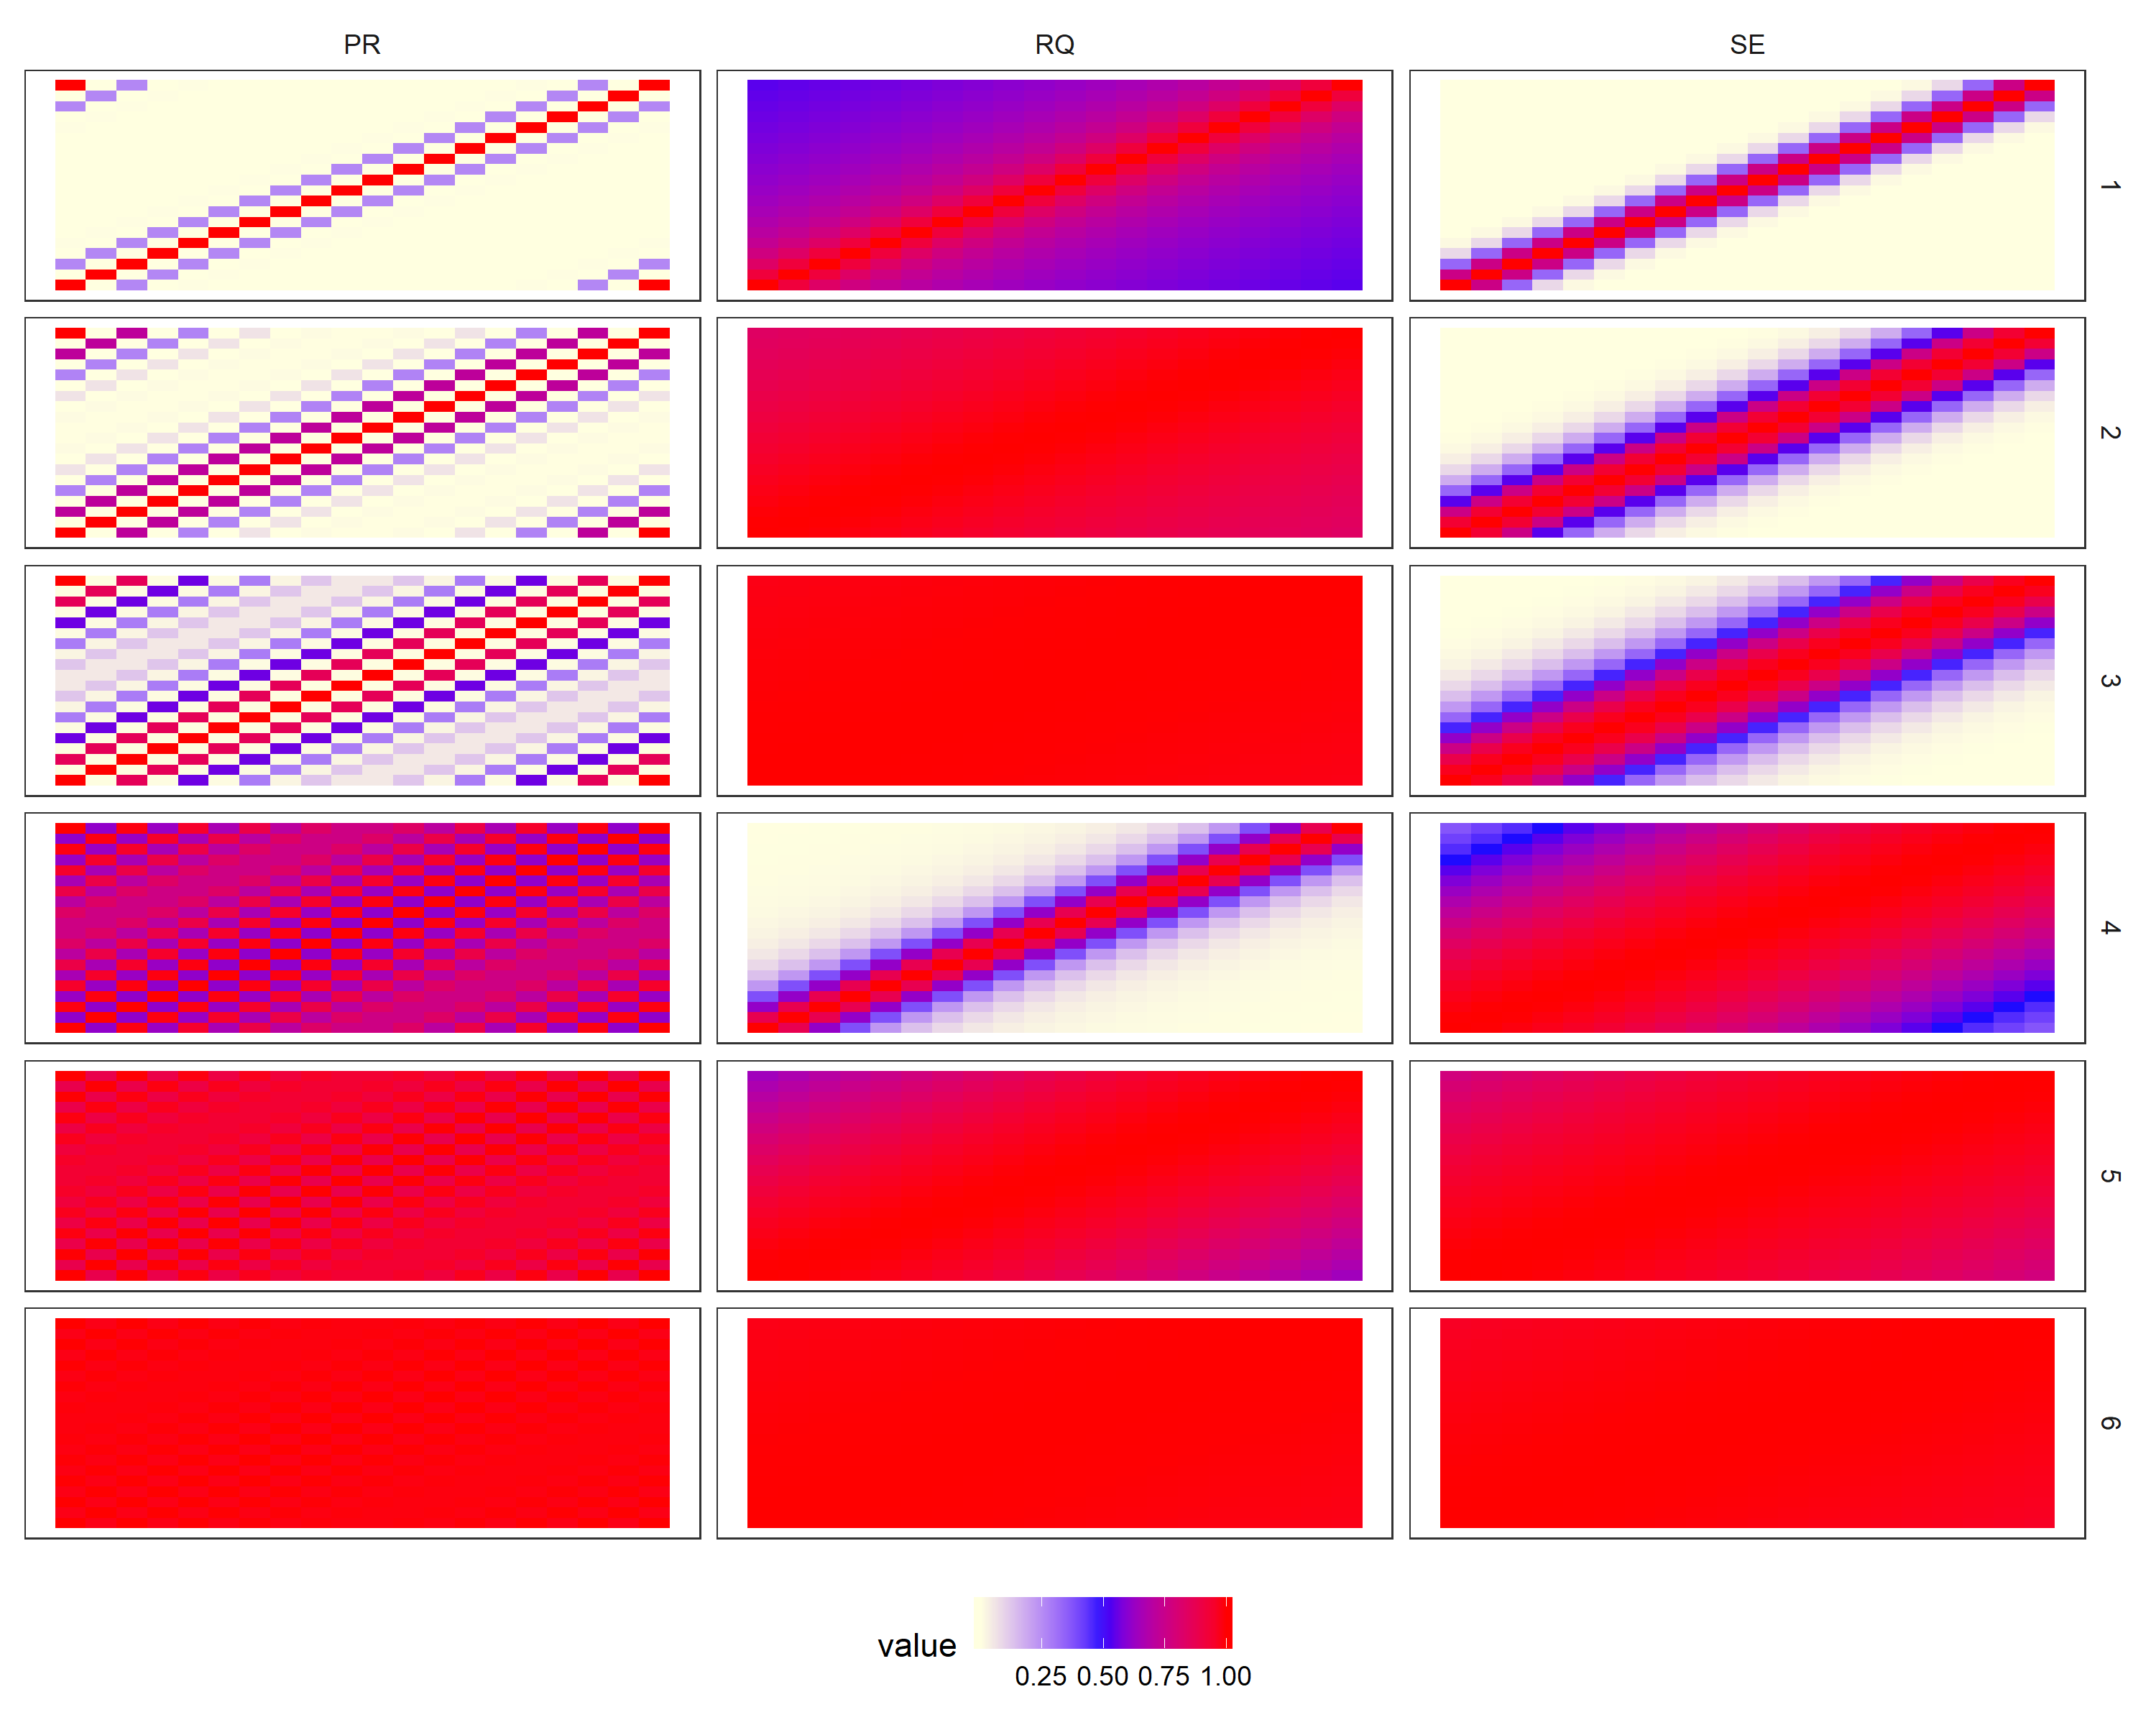
\includegraphics[scale = 0.15]{GP_illustrations/kernel_stationary.png}
\caption{Stationary kernels under 6 different sets of hyper-parameters.}\label{fig:}
\end{figure}

\begin{figure}[H]
\centering
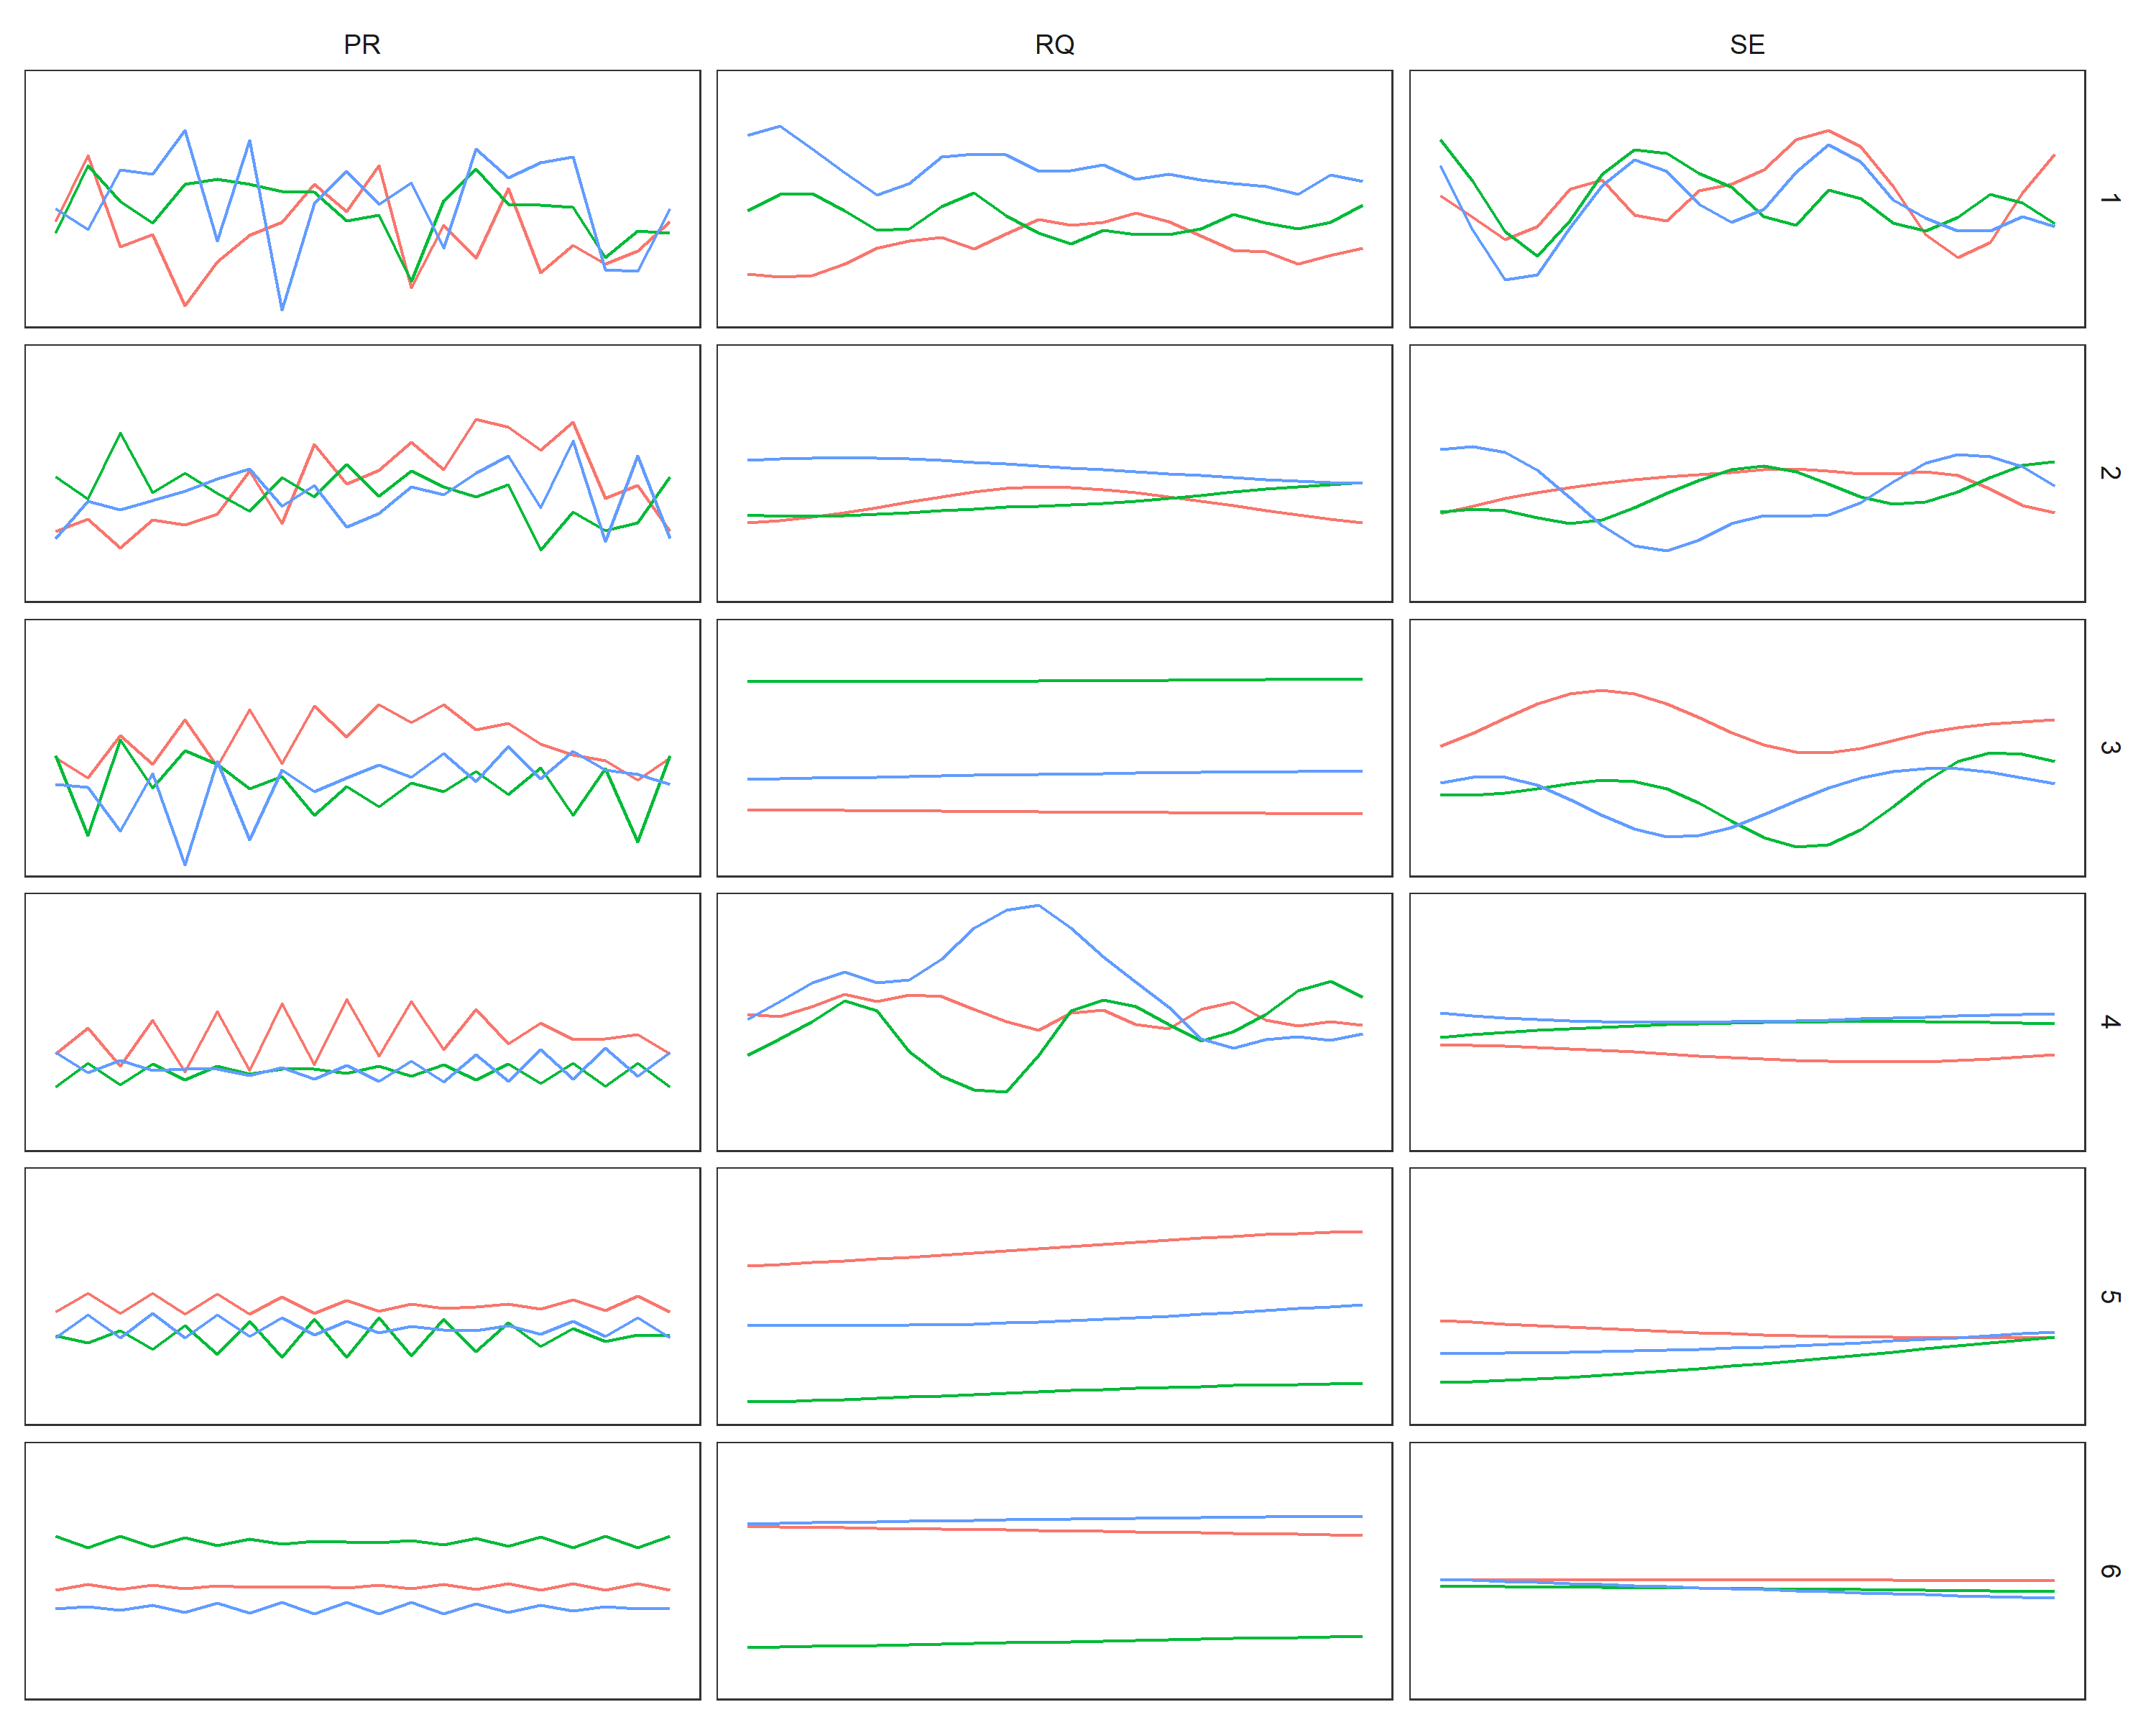
\includegraphics[scale = 0.15]{GP_illustrations/y_sim_stationary.png}
\caption{The 3 path of the signal $c_k$ simulated from the a priori distribution in Equation \eqref{eq:model_IMF_GP_k} under different stationary kernel assumptions (columns wise) and for 6 different sets of hyper-parameters.}\label{fig:}
\end{figure}

\begin{figure}[H]
\centering
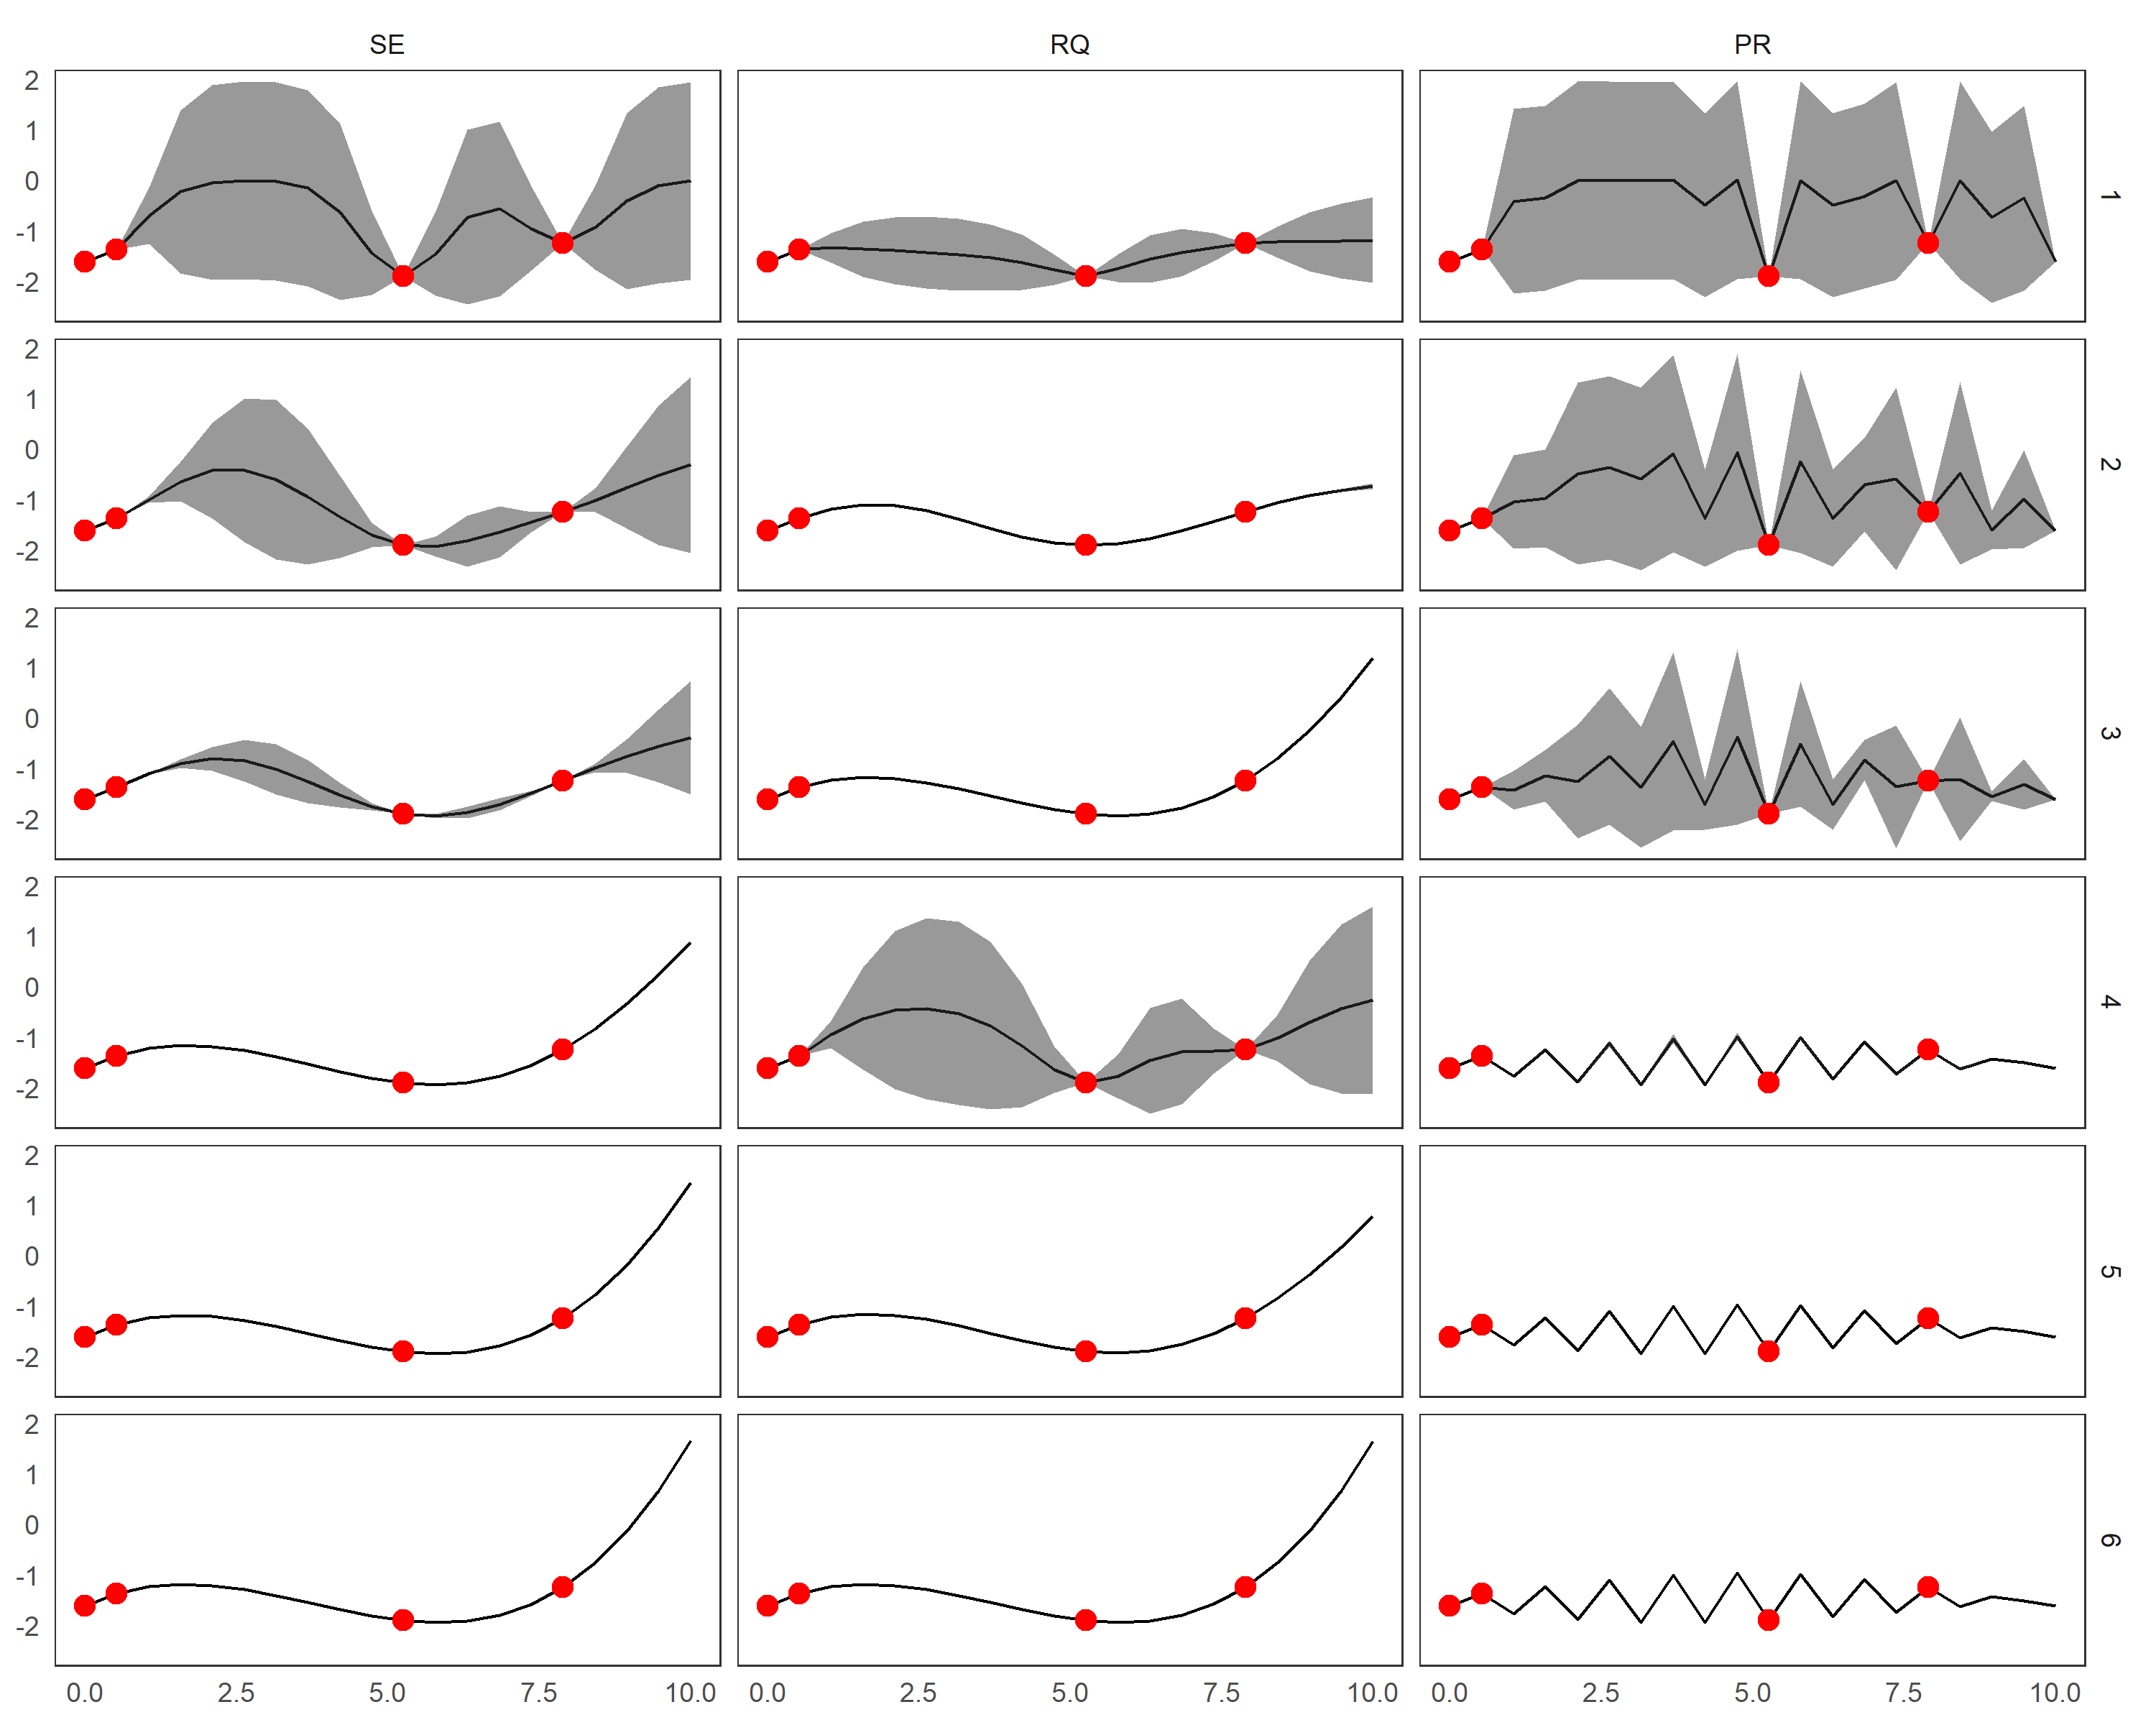
\includegraphics[scale = 0.15]{GP_illustrations/y_pred_stationary.png}
\caption{The predictive conditional mean of the IMF with the confidence intervals  under  noise-free assumption for different stationary kernel assumptions (columns wise) given 6 different sets of hyper-parameters. The red dots correspond to the observed values of the signal}\label{fig:}
\end{figure}